\begin{frame}{Herramientas}
    \begin{block}
        \begin{itemize}
            \item \textbf{C++}: Herramienta principal para el desarrollo de la
                librería.
            \item \textbf{MySQL}: Sirvidor de base de datos utilizada.
            \item Librería \textbf{MySQL Connector/C++}: Sirvidor de base de
                datos utilizada.
            \item \textbf{Otras herramientas}: Apache, PHP, PHPMyAdmin.
        \end{itemize}
    \end{block}
\end{frame}


\begin{frame}{Diagrama de Clases}
\begin{center}
    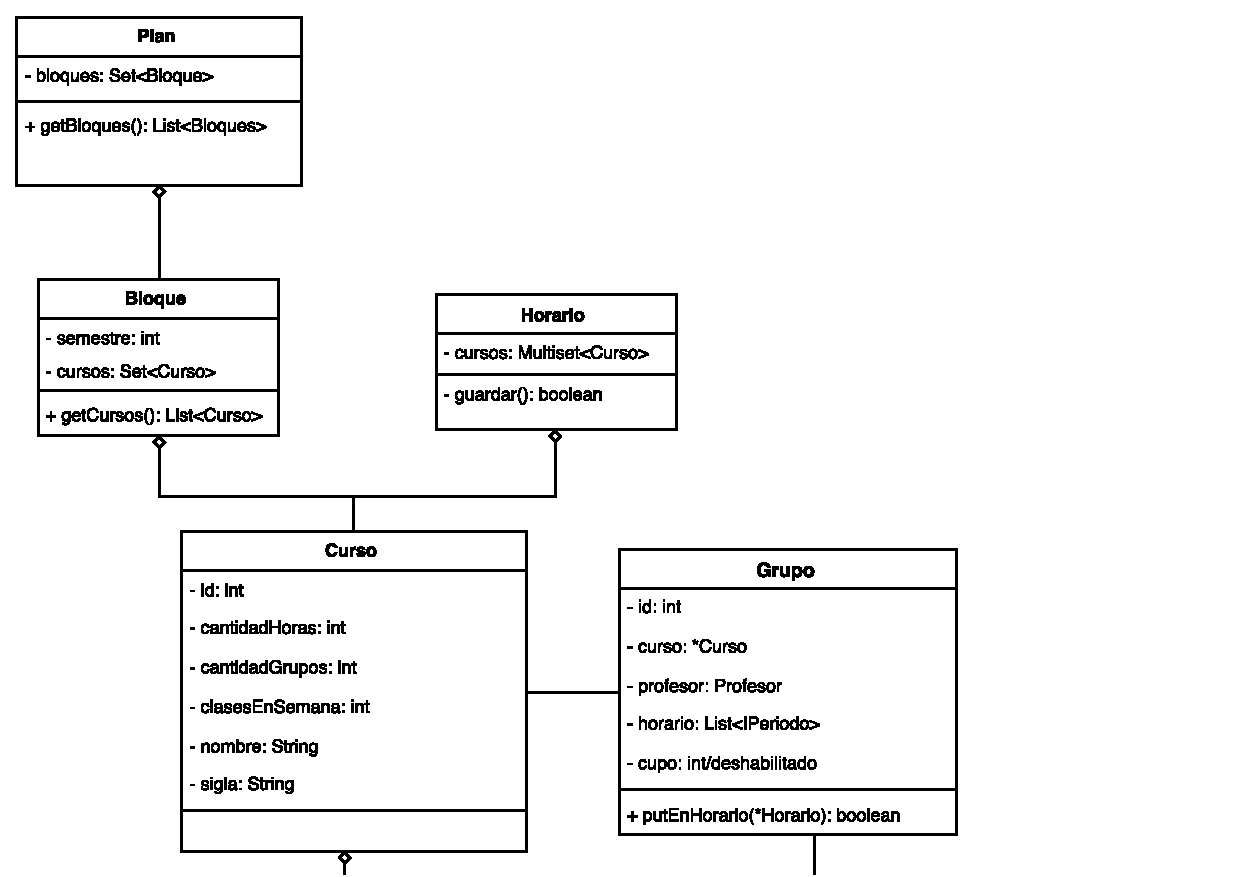
\includegraphics[width=\textwidth]{diagramaClases1}
\end{center}
\end{frame}

\begin{frame}{Diagrama de Clases}
\begin{center}
    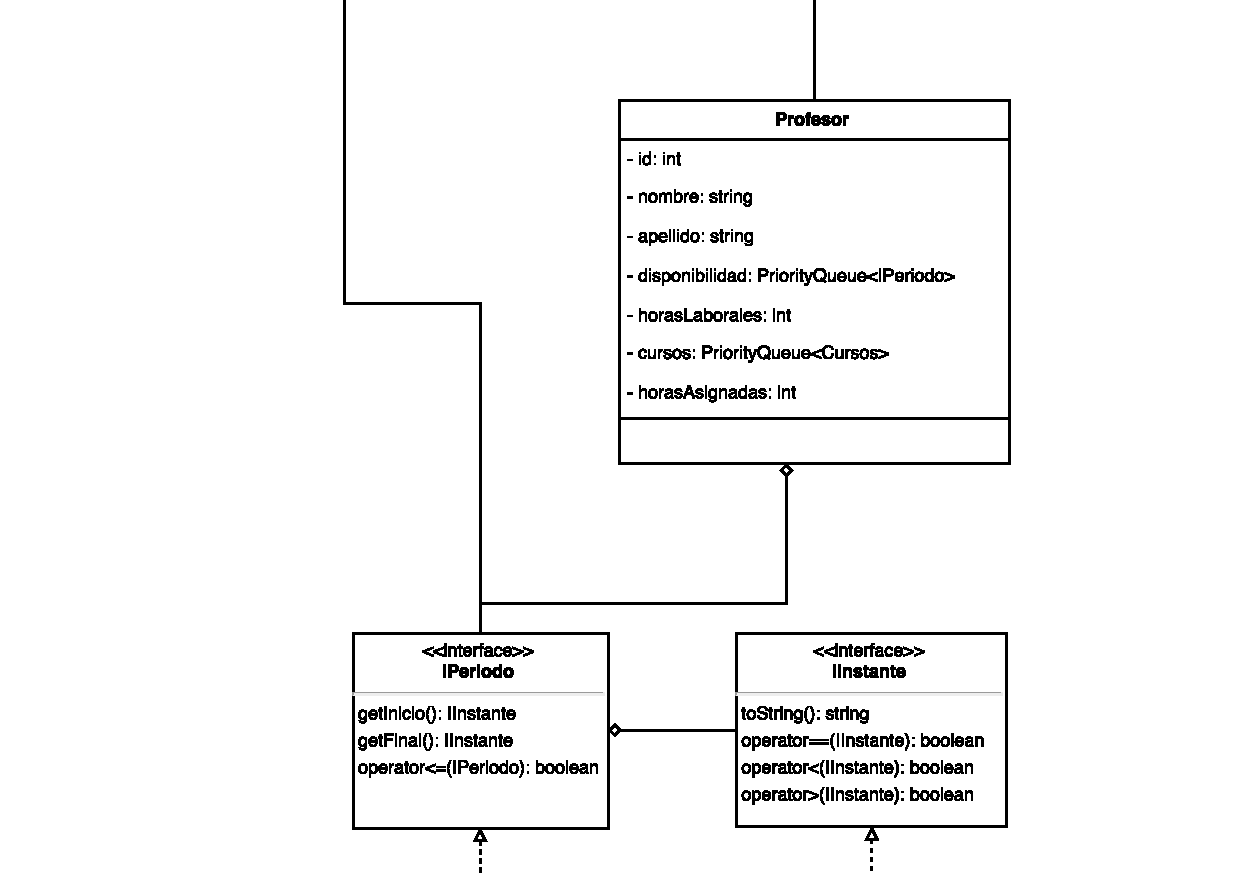
\includegraphics[width=\textwidth]{diagramaClases2}
\end{center}
\end{frame}

\begin{frame}{Diagrama de Clases}
\begin{center}
    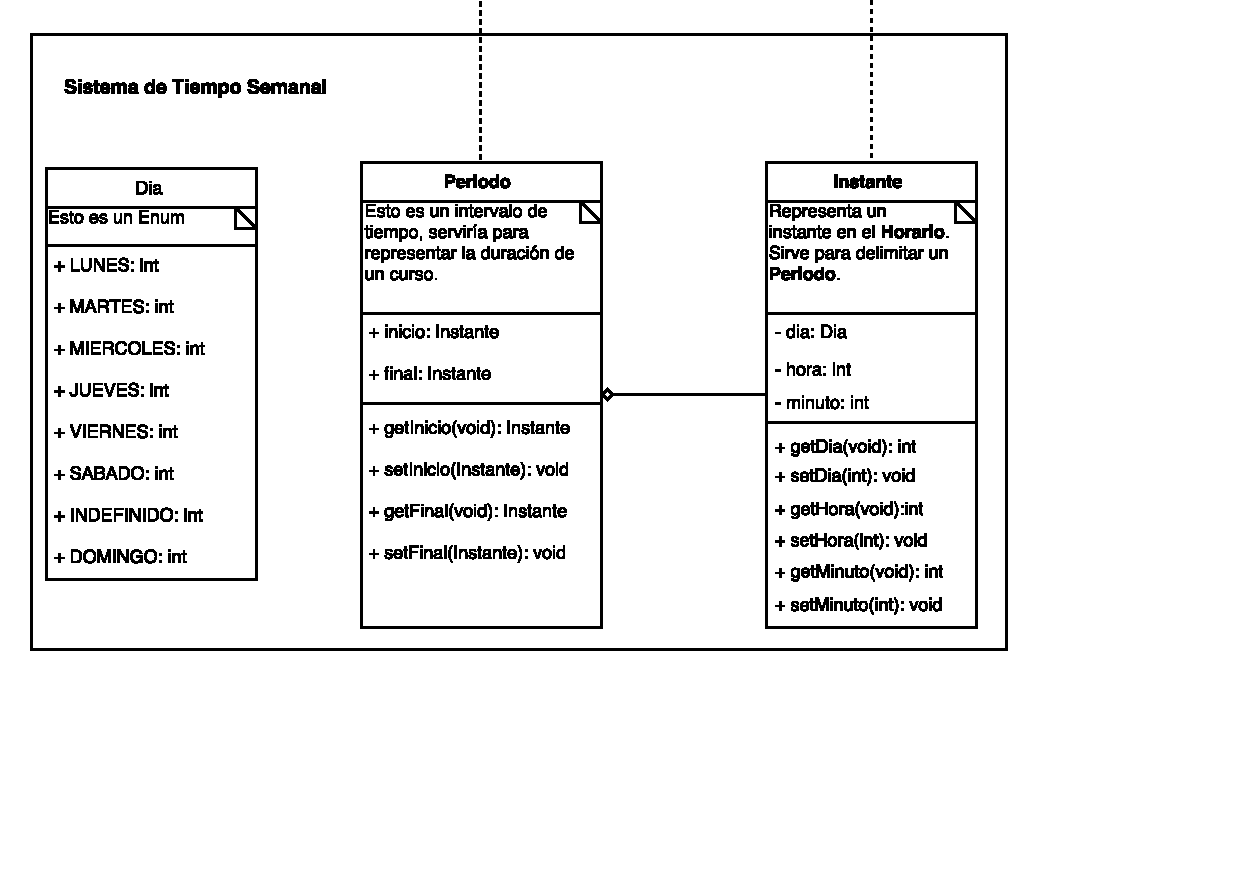
\includegraphics[width=\textwidth]{diagramaClases3}
\end{center}
\end{frame}

\begin{frame}{Logros}
    \begin{itemize}
         \item Declaración de todas las clases.
         \item Creación de la base de datos.
         \item Conexión con la base de datos y btención de resultados a
            consultas.
        \item Implementación de algunas clases y pruebas con estas.
    \end{itemize}
\end{frame}
